\section{Die Anwendung am Beispiel von Bilderkennung}\label{sec:anwendung}

\subsection{Die Problemstellung}\label{subsec:problemstellung}
\begin{wrapfigure}{r}{0.25\textwidth}
    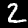
\includegraphics[width=0.25\textwidth]{grafiken/mnist_beispiel}
    \caption[Eins der 70\,000 Bilder der MNIST Datenbank: \textit{MNIST database of handwritten digits}]{Eins der 70\,000 Bilder der MNIST Datenbank}
    \label{fig:mnist-beispiel}
\end{wrapfigure}
Als weitverbreitetes Beispiel zum Training und Testen eines ersten künstlichen neuronalen Netzes wird oft die \textit{MNIST database of handwritten digits} genutzt.
Diese Datenbank enthält 70\,000 verschiedene Graustufen-Bilder mit $28 \times 28$ Pixeln, auf denen jeweils immer eine handgeschriebene Ziffer zwischen 0 und 9 abgebildet ist.
Die MNIST Datenbank hat einen Umfang von 60\,000 Trainings- und 10\,000 Testbildern und deren Bedeutungen als Ziffer.
\autoref{fig:mnist-beispiel} zeigt ein Beispiel für ein solches Bild.
Diese Bilder soll ein selbst trainiertes künstliches neuronales Netzwerk richtig kategorisieren.
Ein KNN wird in der Praxis meist mit anderen Daten trainiert, als mit denen, dessen Genauigkeit getestet wird, da sich so ermitteln lässt, ob das Netz gelernt hat, das gegebene Problem zu lösen oder nur gelernt hat, die Trainingsdaten zu erkennen.
Im Rahmen dieser Arbeit wird für diese Aufgabe ein KNN mit $28 \times 28 = 784$ Eingabeneuronen und 10 Ausgabeneuronen trainiert.
Das Netz hat 784 Eingabeneuronen, da ein Bild, das erkannt werden soll, 784 verschiedene Pixel hat.
Alle Farben eines Pixels liegen zwischen schwarz und weiß, dadurch liegt der Wert eines Eingabeneurons zwischen 0 und 1, wobei alle Farben zwischen schwarz und weiß durch nicht ganze Zahlen zwischen 0 (schwarz) und 1 (weiß) repräsentiert werden.
Auf der letzten Ebene des Netzes befinden sich 10 Neuronen, da es 10 verschiedene Ziffern gibt, die ein KNN einem Bild zuordnen kann.
Je höher der Wert eines Ausgabeneurons, desto höher ist die Sicherheit, die das Netz in diesen Wert als Ergebnis steckt.
Das Ausgabeneuron, welches den höchsten Wert hat, wird als die Entscheidung des Netzes angesehen.
~\footcite{3b1b-3, mnist}

\subsection{Lernrate}\label{subsec:lernrate}
In der Praxis muss das Gradientenverfahren mit einem Faktor reguliert werden, um den Einfluss der mit dem Verfahren ermittelten Werte auf die Variablen des Netzes regulieren zu können.
Diese Konstante nennt sich Lernrate (engl. \textit{Learning rate}) und wird als konstanter Faktor $\eta$ in die Ausdrücke~\eqref{eq:delta-w} und~\eqref{eq:delta-b-neu} integriert, sodass die beiden Ausdrücke folgendermaßen angepasst werden:
\begin{align}
    \Delta w^l_{n p} &= \eta \cdot -\frac{\partial K_d}{\partial w^l_{n p}}
    \label{eq:delta-w-mit-lr}\\
    \Delta b^l_n &= \eta \cdot -\frac{\partial K_d}{\partial z^l_n}
    \label{eq:delta-b-mit-lr}
\end{align}
Beim Wert der Lernrate gilt es, einen Kompromiss zwischen schnellem, aber ungenauem oder langsamem, aber zuverlässigem Lernen zu finden.
Falls die Lernrate zu niedrig eingestellt ist, lernt das Netz gar nicht oder zu langsam.
Falls die Lernrate jedoch zu hoch eingestellt ist, wird während der Anwendung des Gradientenverfahren kein lokales Minimum der Kosten gefunden und das Netz lernt ebenfalls kaum oder nur schlecht.
~\footcite{3b1b-4}

\subsection{Berechnen der Genauigkeit}\label{subsec:genauigkeit}
Um die Zuverlässigkeit eines Netzes vergleichen zu können, gibt es den Wert der Genauigkeit.
Dieser Wert entspricht dem Anteil an richtigen Zuordnungen, die das Netz getroffen hat.
Um die Genauigkeit eines Netzes zu ermitteln, wird das KNN mit den Testdaten getestet und die Anzahl an richtigen Ausgabedaten durch die Anzahl an Testdaten geteilt.
\begin{equation*}
    \frac{Anzahl~an~richtigen~Ausgabedaten}{Anzahl~an~eingegebenen~Daten}
    \label{eq:genauigkeit}
\end{equation*}

\subsection{Vorgehensweise}\label{subsec:vorgehensweise}
Für diesen Teil der Arbeit, habe ich die beschriebenen Verfahren aus \autoref{sec:aufbau} und \autoref{sec:training} mit der Programmiersprache \textit{Rust} in Form eines eigenen Programms implementiert.
Ich habe mich für \textit{Rust} entschieden, da es eine leistungsstarke, schnelle und effiziente Sprache ist.
Leistung und Schnelligkeit sind in diesem Kontext ausschlaggebend, da die Dauer des Trainings stark von der Effizienz der Sprache und der meiner Implementierung abhängig ist.
Im Folgenden wird ein KNN erstellt, welches Bilder von handgeschriebenen Ziffern erkennen soll.
Das von mir dafür verwendete KNN hat zwei Ebenen, was bedeutet, dass es keine verdeckten Ebenen gibt und es nur über eine Eingabe- und Ausgabeebene verfügt.
Ein Netz mit nur zwei Ebenen hat sich in der Praxis als eine bessere Wahl als ein Netz mit mehreren Ebenen herausgestellt.
Beim Erstellen des KNN wird es mit zufälligen Werten für alle Gewichtungen und Biases initialisiert.
Nachdem das Netz initialisiert wurde, wird es mehrmals mit den 60\,000 Trainingsbildern und den dazugehörigen Kennzeichnungen trainiert.
Ein Training mit allen 60\,000 Trainingsbildern wird eine Trainingsepoche genannt.
Ein KNN wird in der Regel, wie auch in meiner Implementierung, mit mehreren Hundert bis Tausend Epochen trainiert.

\subsection{Zuverlässigkeit und Genauigkeit meiner Lösung}\label{subsec:zuverlassigkeit}
Das Trainieren des beschriebenen Netzes in 1\,000 Epochen mit einer Trainingsrate von $\eta = 0,001$ hat 47 Minuten und 10 Sekunden gedauert.
Diese Zeit könnte jedoch noch verkürzt werden, indem nicht jede Epoche die Genauigkeit gespeichert werden würde (siehe \autoref{fig:genauigkeiten-diagramm}).
Nachdem das Training beendet ist, hat das Netz eine Genauigkeit von 92,39\%, da es 9\,239 der 10\,000 Testwerte korrekt kategorisiert hat.
Das bedeutet in der Praxis, dass das Netz zu 92,39\% ein neu eingegebenes Bild, welches es zuvor noch nie gesehen hat, richtig erkennt.\\
\autoref{fig:kosten-diagramm} zeigt die Entwicklung der Kosten während des Trainingsprozesses.
Die x-Achse zeigt die Epochen, während die y-Achse die durchschnittlichen Kosten, die während einer Epoche errechnet wurden, zeigt.
Wie man in \autoref{fig:kosten-diagramm} erkennen kann, waren die Kosten anfangs sehr groß und wurden daraufhin schnell niedriger.
Dieses Verhalten ist dem Gradientenverfahren zuzuschreiben, da es die Variablen des Netzes bei einer starken Abweichung auch stark anpasst.\\
Wie bei \autoref{fig:kosten-diagramm}, liegt bei \autoref{fig:genauigkeiten-diagramm} die Zahl der Epoche auf der x-Achse.
Die y-Achse in \autoref{fig:genauigkeiten-diagramm} zeigt die Genauigkeit des Netzes, angegeben als Anteil zwischen 0 und 1.
Wie auch bei der Entwicklung der Kosten lässt sich hier zu Anfang ein schnelles Verändern der Werte feststellen.
\begin{figure}[h]
    \centering
    \begin{subfigure}{0.45\textwidth}
        \centering
        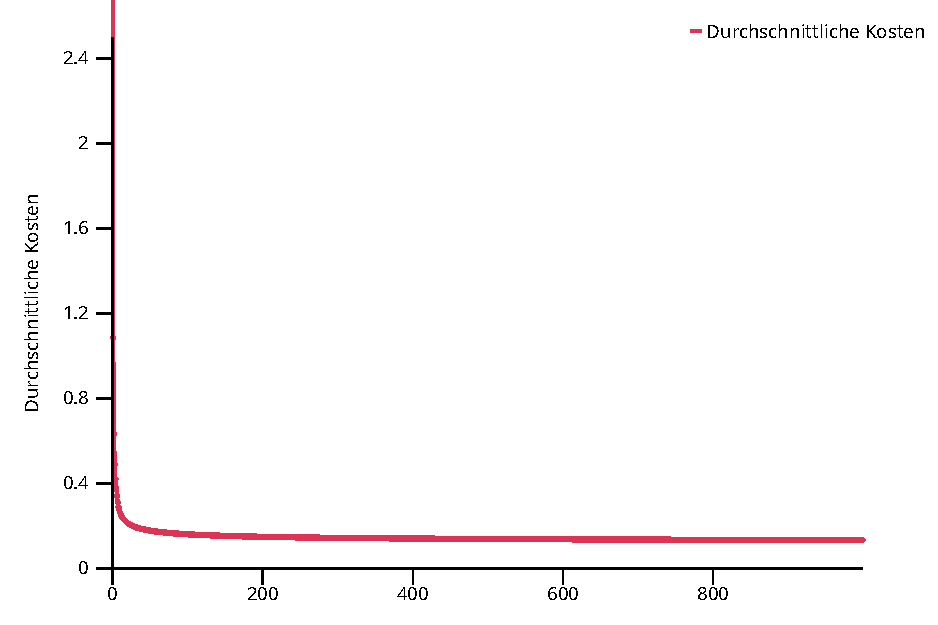
\includegraphics[width=\textwidth]{grafiken/kosten_1000}
        \caption{Entwickelung der Kosten des Netzes während des Trainingsprozesses}
        \label{fig:kosten-diagramm}
    \end{subfigure}
    \begin{subfigure}{0.45\textwidth}
        \centering
        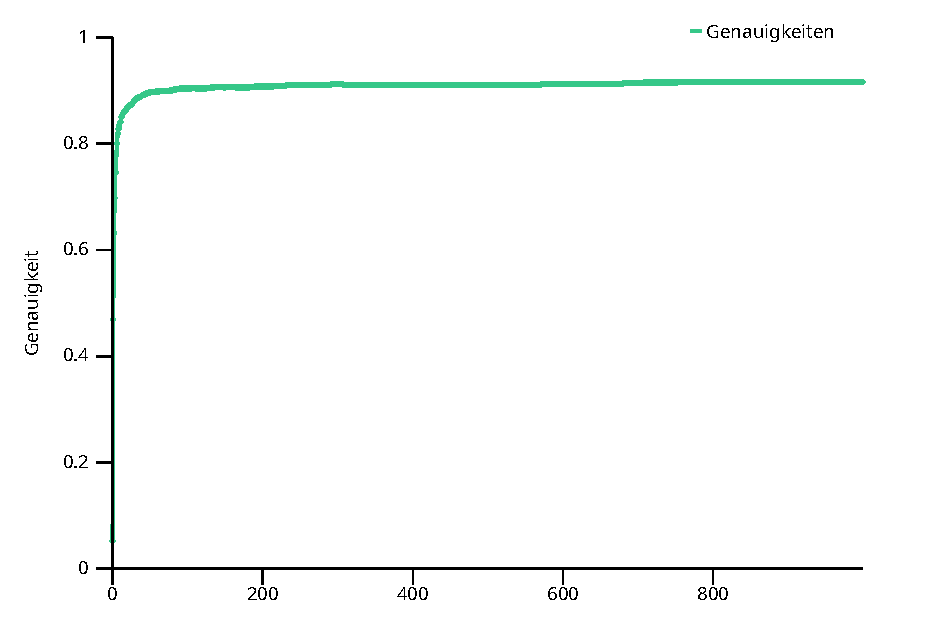
\includegraphics[width=\textwidth]{grafiken/genauigkeiten_1000}
        \caption{Entwickelung der Genauigkeiten des Netzes während des Trainingsprozesses}
        \label{fig:genauigkeiten-diagramm}
    \end{subfigure}
    \caption[Entwickelung der Kosten und Genauigkeiten während des Trainings: \textit{Eigene Grafik, erstellt mit plotlib für Rust}]{}
\end{figure}